\subsection{Technologiewahl Anhang} 

\subsubsection{Stimmen verwendeter Frameworks} 

\begin{figure}[H]
	\centering
    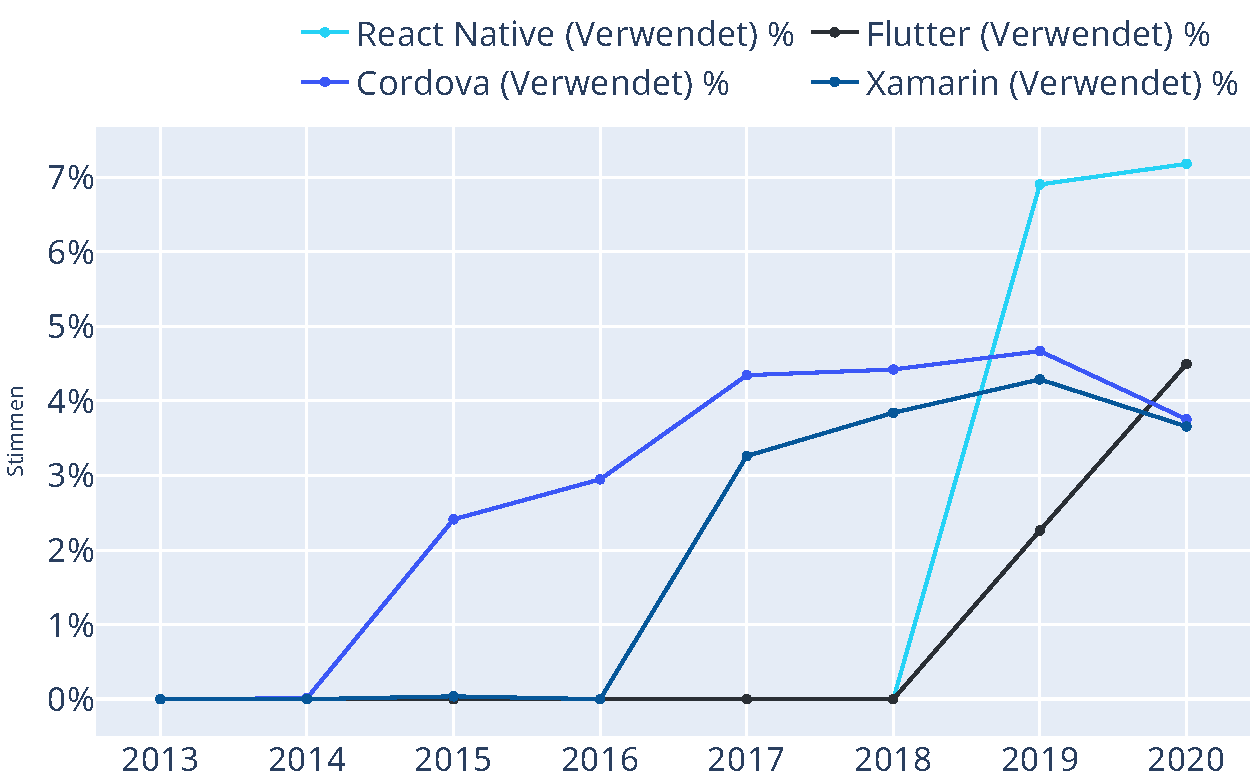
\includegraphics[width=1.0\textwidth]{Charts/Stack Overflow Umfrage/Stimmen verwendeter Frameworks.pdf}
	\caption[Stimmen verwendeter Frameworks]{Stimmen verwendeter Frameworks, Quelle: Eigene Abbildung, Notebook: Charts/Stack Overflow Umfrage/Stack Overflow Umfrage.ipynb}
	\label{fig:StimmenVerwendeter Frameworks}
\end{figure}


\subsubsection{Stimmen gewünschter Frameworks} 

\begin{figure}[H]
	\centering
    \includegraphics[width=1.0\textwidth]{Charts/Stack Overflow Umfrage/Stimmen gewünschter Frameworks.pdf}
	\caption[Stimmen gewünschter Frameworks]{Stimmen gewünschter Frameworks, Quelle: Eigene Abbildung, Notebook: Charts/Stack Overflow Umfrage/Stack Overflow Umfrage.ipynb}
	\label{fig:StimmenGewuenschterFrameworks}
\end{figure}





\subsection{Vergleich React Native und Flutter Anhang} 


\begin{listing}[H]
	\label{lst:quelltext1}

    \begin{minted}[
        linenos, % Quelltextzeilen anzeigen
        numbersep=5pt, %Abstand
        firstnumber=1,
        frame=lines,
        fontsize=\small,
        framesep=2mm,
		tabsize=4,
		breaklines,
		breakafter=_@|
        ]{dart}
import 'package:flutter/material.dart';
import 'input.dart';

void main() => runApp(MyApp());

class MyApp extends StatelessWidget {
  @override
  Widget build(BuildContext context) => MaterialApp(
		home: Scaffold(
		  body: MyCustomForm(),
		),
	  );
}

final emailPattern = new RegExp(
    r'^(([^<>()\[\]\\.,;:\s@\enquote{]+(\.[^<>()\[\]\\.,;:\s@} ]+)*)|(\enquote{.+} ))@((\[[0-9]{1,3}\.[0-9]{1,3}\.[0-9]{1,3}\.[0-9]{1,3}\])|(([a-zA-Z\-0-9]+\.)+[a-zA-Z]{2,}))$');

class MyCustomForm extends StatefulWidget {
  @override
  MyCustomFormState createState() => MyCustomFormState();
}

class MyCustomFormState extends State<MyCustomForm> {
  final _formKey = GlobalKey<FormState>();

  @override
  Widget build(BuildContext context) => Form(
		key: _formKey,
		child: Padding(
		  padding: const EdgeInsets.all(8.0),
		  child: Column(
			children: [
			  Input(label: \enquote{Name} ),
			  Input(
				  label: \enquote{Email} ,
				  validator: (value) {
					if (value == null || !emailPattern.hasMatch(value)) {
					  return 'Invalid Email Format';
					}
					return null;
				  }),
			  Input(label: \enquote{Password} ),
			  Padding(
				padding: const EdgeInsets.symmetric(vertical: 16.0),
				child: ElevatedButton(
				  onPressed: () {
					if (_formKey.currentState!.validate()) {
					  ScaffoldMessenger.of(context).showSnackBar(
						  SnackBar(content: Text('Processing Data')));
					}
				  },
				  child: Text('Submit'),
				),
			  ),
			],
		  ),
		),
	  );
}
		
    \end{minted}

    \caption[main.dart]{main.dart Datei}
\end{listing}


\begin{listing}[H]
	\label{lst:quelltext2}

    \begin{minted}[
        linenos, % Quelltextzeilen anzeigen
        numbersep=5pt, %Abstand
        firstnumber=1,
        frame=lines,
        fontsize=\small,
        framesep=2mm,
		tabsize=4,
		breaklines,
		breakafter=_@|
        ]{javascript}
export default {
	name: {required: {value: true, message: 'Name is required'}},
	email: {
	  required: {value: true, message: 'Email is required'},
	  pattern: {
		value: /^(([^<>()\[\]\\.,;:\s@\enquote{]+(\.[^<>()\[\]\\.,;:\s@} ]+)*)|(\enquote{.+} ))@((\[[0-9]{1,3}\.[0-9]{1,3}\.[0-9]{1,3}\.[0-9]{1,3}\])|(([a-zA-Z\-0-9]+\.)+[a-zA-Z]{2,}))$/,
		message: 'Invalid Email Format',
	  },
	},
	password: {
	  required: {value: true, message: 'Password is required'},
	},
  };
    \end{minted}

    \caption[validation.tsx]{validation.tsx Datei}
\end{listing}


\begin{listing}[H]
	\label{lst:quelltext3}

    \begin{minted}[
        linenos, % Quelltextzeilen anzeigen
        numbersep=5pt, %Abstand
        firstnumber=1,
        frame=lines,
        fontsize=\small,
        framesep=2mm,
		tabsize=4,
		breaklines,
		breakafter=_@|
        ]{dart}
final emailPattern = new RegExp(
	r'^(([^<>()\[\]\\.,;:\s@\enquote{]+(\.[^<>()\[\]\\.,;:\s@} ]+)*)|(\enquote{.+} ))@((\[[0-9]{1,3}\.[0-9]{1,3}\.[0-9]{1,3}\.[0-9]{1,3}\])|(([a-zA-Z\-0-9]+\.)+[a-zA-Z]{2,}))$');

validateEmail(value) {
  if (value == null || !emailPattern.hasMatch(value))
	return 'Invalid Email Format';
  else
	return null;
}

validateNotEmpty(String label, value) {
  if (value == null || value.isEmpty)
	return '$label is required';
  else
	return null;
}		
    \end{minted}

    \caption[validation.dart]{validation.dart Datei}
\end{listing}


\begin{listing}[H]
	\label{lst:quelltext4}

    \begin{minted}[
        linenos, % Quelltextzeilen anzeigen
        numbersep=5pt, %Abstand
        firstnumber=1,
        frame=lines,
        fontsize=\small,
        framesep=2mm,
		tabsize=4,
		breaklines,
		breakafter=_@|
        ]{dart}
import 'package:example_form_app/validation.dart';
import 'package:flutter/material.dart';

class Input extends StatelessWidget {
  final String label;
  final FormFieldValidator<String>? validator;

  const Input({required this.label, this.validator});

  @override
  Widget build(BuildContext context) => TextFormField(
	  decoration: InputDecoration(labelText: label),
	  validator: validator ?? (value) => validateNotEmpty(label, value));
}
    \end{minted}

    \caption[input.dart]{input.dart Datei}
\end{listing}













\begin{listing}[H]
	\label{lst:quelltext5}

    \begin{minted}[
        linenos, % Quelltextzeilen anzeigen
        numbersep=5pt, %Abstand
        firstnumber=1,
        frame=lines,
        fontsize=\small,
        framesep=2mm,
		tabsize=4,
		breaklines,
		breakafter=_@|
        ]{javascript}
import * as React from 'react';
import { TextInput, KeyboardAvoidingView, findNodeHandle } from 'react-native';
import { ValidationOptions, FieldError } from 'react-hook-form';

interface ValidationMap {
  [key: string]: ValidationOptions;
}

interface ErrorMap {
  [key: string]: FieldError | undefined;
}

interface Props {
  children: JSX.Element | JSX.Element[];
  register: (
    field: { name: string },
    validation?: ValidationOptions
  ) => void;
  errors: ErrorMap;
  validation: ValidationMap;
  setValue: (name: string, value: string, validate?: boolean) => void;
}
\end{minted}


\caption[Form.tsx]{Form.tsx Datei}
\end{listing}

\begin{listing}[H]
	\label{lst:quelltext6}
    \inputminted[lastline=23, linenos, numbersep=5pt, firstnumber=1, frame=lines, fontsize=\small, framesep=2mm, tabsize=4, breaklines, breakafter=_@|]
    {typescript}
    {source_code/flutter_vs_react_native/react_native/example_form_app/form-in-react-native-the-right-way/components/Form.tsx}
\caption[Form.tsx]{Form.tsx Datei}
\end{listing}
 
\begin{listing}[H]
	\label{lst:quelltext7}
    \inputminted[firstline=24, linenos, numbersep=5pt, firstnumber=24, frame=lines, fontsize=\small, framesep=2mm, tabsize=4, breaklines, breakafter=_@|]
    {typescript}
    {source_code/flutter_vs_react_native/react_native/example_form_app/form-in-react-native-the-right-way/components/Form.tsx}
\caption[Form.tsx]{Form.tsx Datei}
\end{listing}




\begin{listing}[H]
	\label{lst:quelltext8}
    \begin{minted}[
        linenos, % Quelltextzeilen anzeigen
        numbersep=5pt, %Abstand
        firstnumber=1,
        frame=lines,
        fontsize=\small,
        framesep=2mm,
		tabsize=4,
		breaklines,
		breakafter=_@|
        ]{javascript}
import * as React from 'react';
import {
  View,
  TextInput,
  Text,
  StyleSheet,
  ViewStyle,
  TextStyle,
  TextInputProps,
} from 'react-native';
import { FieldError } from 'react-hook-form';
interface Props extends TextInputProps {
  name: string;
  label?: string;
  labelStyle?: TextStyle;
  error?: FieldError | undefined;
}

export default React.forwardRef<any, Props>(
  (props, ref): React.ReactElement => {
	const { label, labelStyle, error, ...inputProps } = props;

	return (
	  <View style={styles.container}>
		{label && <Text style={[styles.label, labelStyle]}>{label}</Text>}
		<TextInput
		  autoCapitalize=\enquote{none}
		  ref={ref}
		  style={[styles.input, { borderColor: error ? '#fc6d47' : '#c0cbd3' }]}
		  {...inputProps}
		/>
		<Text style={styles.textError}>{error && error.message}</Text>
	  </View>
	);
  }
);

const styles = StyleSheet.create({
  container: {
	marginVertical: 8,
  },
  input: {
	borderWidth: 1,
	paddingLeft: 5,
  },
  label: {
	paddingVertical: 5,
  },
  textError: {
	color: '#fc6d47',
  },
});	
\end{minted}


\caption[Input.tsx]{Input.tsx Datei}
\end{listing}


 

\begin{listing}[H]
	\label{lst:quelltext9}

    \begin{minted}[
        linenos, % Quelltextzeilen anzeigen
        numbersep=5pt, %Abstand
        firstnumber=1,
        frame=lines,
        fontsize=\small,
        framesep=2mm,
		tabsize=4,
		breaklines,
		breakafter=_@|
        ]{javascript}
import * as React from 'react';
import {
  Text,
  View,
  StyleSheet,
  Button,
  Alert,
  ScrollView,
} from 'react-native';

import { useForm } from 'react-hook-form';

import Input from './components/Input';
import Form from './components/Form';
import validation from './validation';

type FormData = {
  name: string;
  email: string;
  password: string;
};

export default () => {
  const { handleSubmit, register, setValue, errors } = useForm<FormData>();

  const onSubmit = (data: FormData) => {
	Alert.alert('data', JSON.stringify(data));
  };

  return (
	  <View style={styles.formContainer}>
		<Form {...{ register, setValue, validation, errors }}>
		  <Input name=\enquote{name} label=\enquote{Name } />
		  <Input name=\enquote{email} label=\enquote{Email} />
		  <Input name=\enquote{password} label=\enquote{Password} secureTextEntry={true} />
		  <Button title=\enquote{Submit} onPress={handleSubmit(onSubmit)} />
		</Form>
	  </View>
  );
};

const styles = StyleSheet.create({
  formContainer: {
	padding: 8,
	flex: 1,
  }
});		
\end{minted}


\caption[App.tsx]{App.tsx Datei}
\end{listing}
